\subsection{Existing Models}
Necessary requirements are elaborated and graded on every drone. As this comparison is purely about the performance of the drone for the project, no attention is given to price until after this comparison. Options for acquiring the drone will be briefly discussed.

\subsubsection{Grading} \label{grading}
Drones are graded by a product of their requirements. They start out with a score of 1. Each of these requirements are graded by rational number from 0-1.5. This way, a requirement score of 1.2 can positively affect the end grade, while a requirement score of 0 dismisses the drone all together. 

This makes it possible to easily disregard a drone when it does not meet a requirement at all. Care must be put in dismissing drones though, since there sometimes exist alternatives that can fix these requirements. Generally, any drone above a score of 1 can be suitable for the project. 

\subsubsection{Overview of the requirements}
In this section, an overview of the requirements are given, including minimal values for these requirements. Further explanation might be given about different solutions that might exist to reach these requirements. 

\paragraph{Payload capacity}\mbox{} \\
The payload capacity is the maximum amount of weight a drone can safely carry while flying. While exceeding the payload capacity by a bit is often possible, it is never encouraged by the manufacturer. A large payload can shift the center of mass too much for the drone's stabilization to work reliably. There are also physical limits to the combined lifting force of the rotors. Summing up the weight of potential sensors of the drone, it is expected that the minimum payload capacity on paper should be 500g.

\paragraph{Mounting clearance}\mbox{} \\
There are several ways to mount sensors on a drone. Some drones have dedicated mounting holes while others rely on the user to come up with their own solution. There must be enough clearance on the bottom of the drone for the sensors to mount on. The amount of clearance could sometimes be extended by modifying the drone.

\paragraph{Navigation/Routing}\mbox{} \\
The drone must be able to navigate on its own to multiple previously marked GPS locations and return to home. Some drones have this functionality built into their own app, others don't even have an app. When this functionality isn't built in, it could be developed or the drone could be integrated into an open source software suite like ArduPilot \cite{ardupilot} if a SDK is available. This would delay the development cycle.
\newpage
\paragraph{Flight time}\mbox{} \\
The drone ideally should be able to take multiple measurements per flight. Care should be taken when looking at flight times at data sheets, as these often don't include flight time whenever the drone has payload. The longer the flight time the better, a minimum of 10 minutes flight time should be fine.

\paragraph{Range}\mbox{} \\
Often there are two different ranges included in datasheets, the image transmission range and the drone operating radio range. In this project, real time transmission of images has a low priority, so the focus is laid on operating radio range. Again, care should be taken whenever looking at range as data sheets usually report this range without obstructions. Thankfully, as there are little obstructions in the Mekong Delta, the realistic range would be very similar. A minimum of 1 kilometer operating range is required.

\paragraph{Waterproof}\mbox{} \\
It is important to reduce the risk of damaging the drone as much as possible. As the measurements takes place near and on water, using a waterproof drone is vital. Generally, drones denote the level of solid and liquid protection by the Ingress Protection standard. The IP standard classifies the degree of protection provided by an enclosure. \cite{ipstandard} For this project, a minimum rating of IP64 would be sufficient, meaning dust-tight and resistant against splashes of water.

For drones that are not waterproof, certain wet suits are available to alleviate this issue. \cite{phantomrain}

\paragraph{Landing in water}\mbox{} \\
For some measurements and emergency landings it is best that the drone is able to land in the water. While there are not a lot of drones available that have this feature out of the box, there is some commercial water landing gear available.\cite{buylanding} Designing your own landing gear is also possible. \cite{diylanding} Water landing gear often also increase the amount of clearance available for sensors.

\paragraph{Maneuverability}\mbox{} \\
The drone should not get stuck on it's flight in the Mekong River. It should be fast enough to take the measurements, and it should be stable enough to be used in an autonomous environment. These aspects are what determines the maneuverability of the drone.

\newpage
\subsubsection{Swellpro SplashDrone 4}
\begin{wrapfigure}{r}{0.3\textwidth}
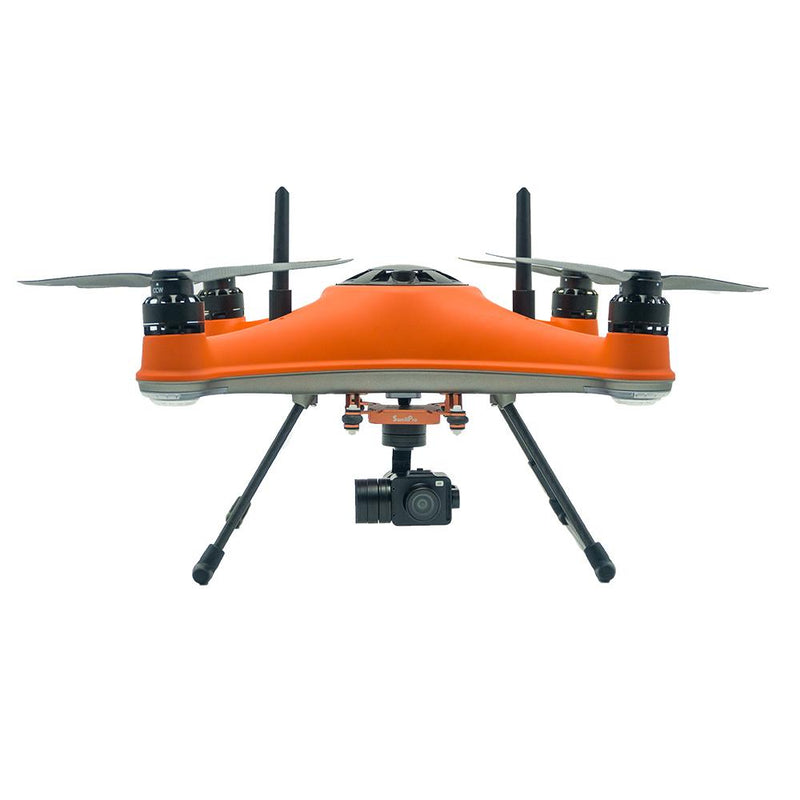
\includegraphics[width=1\linewidth]{uav/models/01_splashdrone4.png}
\caption{SplashDrone 4}
\end{wrapfigure}
The SplashDrone 4 \cite{splashdrone4} is Swellpro's flagship drone. It is fully designed to be used in the water.

\paragraph{Payload capacity}\mbox{Score: 1.5} \\
The payload capacity of the SplashDrone 4 is 2kg, enough for all of our gear.

\paragraph{Mounting clearance}\mbox{Score: 1.3} \\
The SplashDrone 4 is a medium compact drone and therefore doesn't have a lot of clearance for sensors. It does have mounting holes for payloads at the bottom of the drone, which make mounting sensors easy. The drone can also flip over in the water, so one could also manually mount sensors on top of the drone. Additionally, Swellpro sells a water collector for the Splashdrone 4 to take water samples. \cite{watercollector}

\paragraph{Navigation/Routing}\mbox{Score: 1.5} \\
One can plan routes for the SplashDrone 4 using the SwellPro SDFly App. The app has support for waypoint mission planning and grid mission planning. Additionally, a SDK and API is also in development for when one wants to create their own add-ons or flight platform.

\paragraph{Flight time}\mbox{Score: 1.5} \\
The flight time of the SplashDrone 4 is 30 minutes, well over the minimum required flight time.

\paragraph{Range}\mbox{Score: 1.5} \\
The maximum radio range is 5.0km, well over the minimum required range. This also includes image transmission.

\paragraph{Waterproof}\mbox{Score: 1.5} \\
The drone is IP67 waterproof, meaning the drone is dust-tight and can immerse up to 1 meter in water. This is well over the minimum required IP rating.

\paragraph{Landing in water}\mbox{Score: 1.5} \\
The drone is designed to land and take off in the water.

\paragraph{Maneuverability}\mbox{Score: 1.4} \\
When the drone turns upside down on the water for any reason, it automatically turns the drone back around to the normal state. It can fly horizontally 10m/s with the GPS being the limiting factor.

\paragraph{Total score:}\mbox{20.7} \\
The SplashDrone 4 seems to be a very adequate system for the project, with it's extensible and water-first design.
\newpage
\subsubsection{Swellpro Fisherman FD1}
\begin{wrapfigure}{r}{0.3\textwidth}
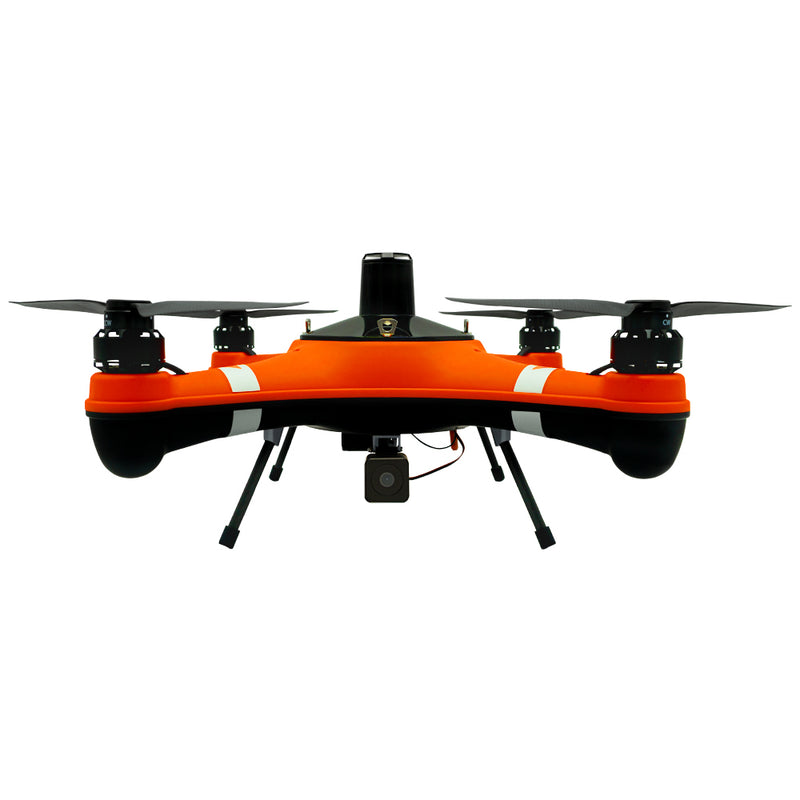
\includegraphics[width=1\linewidth]{uav/models/11_fishermanfd1.png}
\caption{Fisherman FD1}
\end{wrapfigure}
The Fisherman FD1 \cite{fishermanfd1} is Swellpro's economical offering based on their previous flagship. It is also fully designed to be used in the water.

\paragraph{Payload capacity}\mbox{Score: 1.5} \\
The payload capacity of the Fisherman FD1 is 2kg, well above the minimum requirement.

\paragraph{Mounting clearance}\mbox{Score: 1.1} \\
The Fisherman FD1 is a medium compact drone and therefore doesn't have a lot of clearance for sensors. One could create their own platform beneath the drone, utilizing the four feet.

\paragraph{Navigation/Routing}\mbox{Score: 0.5} \\
While the Fisherman FD1 is based off of the SplashDrone 3+ that has an app that allows waypoints, it is not clear if this revised version can use that app as well. One might need to acquire a remote from the SplashDrone 3+ for the app to work.
As an alternative, one could hack into the internals of the drone with relative ease and use an open source flight system like ArduPilot.

\paragraph{Flight time}\mbox{Score: 1.5} \\
The flight time of the SplashDrone 4 is 30 minutes, well over the minimum required flight time.

\paragraph{Range}\mbox{Score: 1.2} \\
The maximum radio range is 1.6km, passing the minimum required range. This includes image transmission.

\paragraph{Waterproof}\mbox{Score: 1.5} \\
The drone is IP67 waterproof, meaning the drone is dust-tight and can immerse up to 1 meter in water. This is well over the minimum required IP rating.

\paragraph{Landing in water}\mbox{Score: 1.5} \\
The drone is designed to land and take off in the water.

\paragraph{Maneuverability}\mbox{Score: 1.1} \\
The drone can fly horizontally 10m/s with the GPS being the limiting factor.

\paragraph{Total score:}\mbox{3.7} \\
The Fisherman FD1 looks like a capable budget-friendly alternative to the SplashDrone 4, but the compatibility of the waypoint app needs to be figured out.


\newpage
\subsubsection{Swellpro Spry+}
\begin{wrapfigure}{r}{0.3\textwidth}
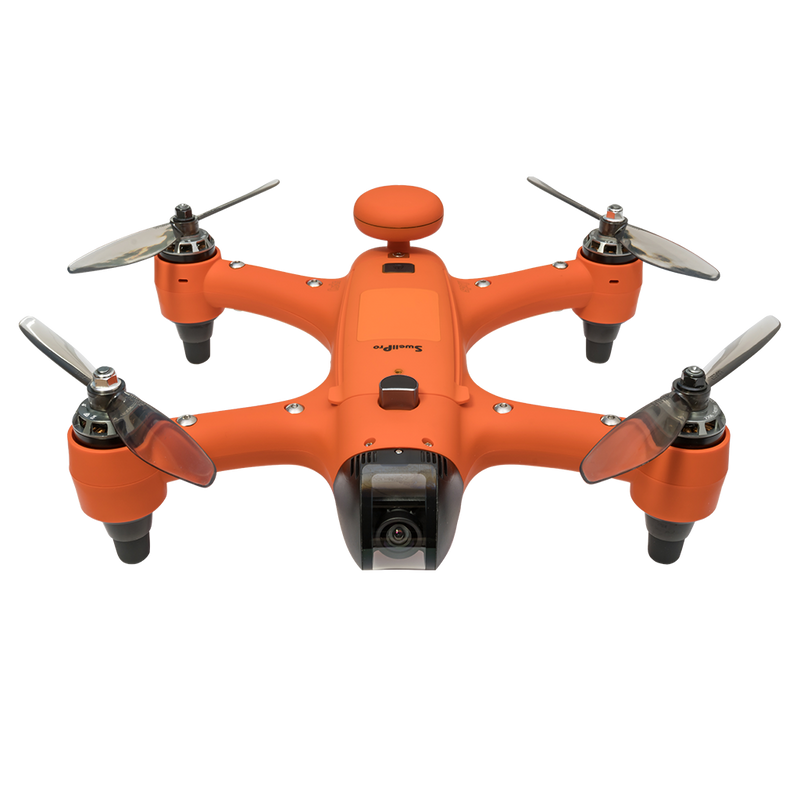
\includegraphics[width=1\linewidth]{uav/models/21_spry.png}
\caption{Spry+}
\end{wrapfigure}
The Spry+ \cite{spry} is Swellpro's action drone. It is also fully designed to be used in the water.

\paragraph{Payload capacity}\mbox{Score: 0} \\
While the payload capacity of the Spry+ is not presented on the website, professionals state that the drone can carry up to 300g\cite{sprypayload}. This is below the minimum required payload of 500g.

\paragraph{Mounting clearance}\mbox{Score: 0.8} \\
The Spry+ is a compact drone meant for speed and therefore lacks clearance for sensors. One could create their own platform beneath the drone, utilizing the four bars.

\paragraph{Navigation/Routing}\mbox{Score: 1.4} \\
One can plan routes for the Spry+ using the SwellPro Spry App. The app has support for waypoint mission planning.

\paragraph{Flight time}\mbox{Score: 1.5} \\
The flight time of the SplashDrone 4 is 15 minutes, passing the minimum required flight time.

\paragraph{Range}\mbox{Score: 0} \\
The maximum radio range is 800m, failing the minimum required range.

\paragraph{Waterproof}\mbox{Score: 1.5} \\
The drone is IP67 waterproof, meaning the drone is dust-tight and can immerse up to 1 meter in water. This is well over the minimum required IP rating.

\paragraph{Landing in water}\mbox{Score: 1.5} \\
The drone is designed to land and take off in the water.

\paragraph{Maneuverability}\mbox{Score: 1.5} \\
The drone can fly horizontally 18m/s. It is designed for high speed movement.

\paragraph{Total score:}\mbox{0} \\
Due to the Spry+ being an action drone it wasn't able to meet the range and payload capacity requirements.


\newpage
\subsubsection{PowerEgg X}
\begin{wrapfigure}{r}{0.3\textwidth}
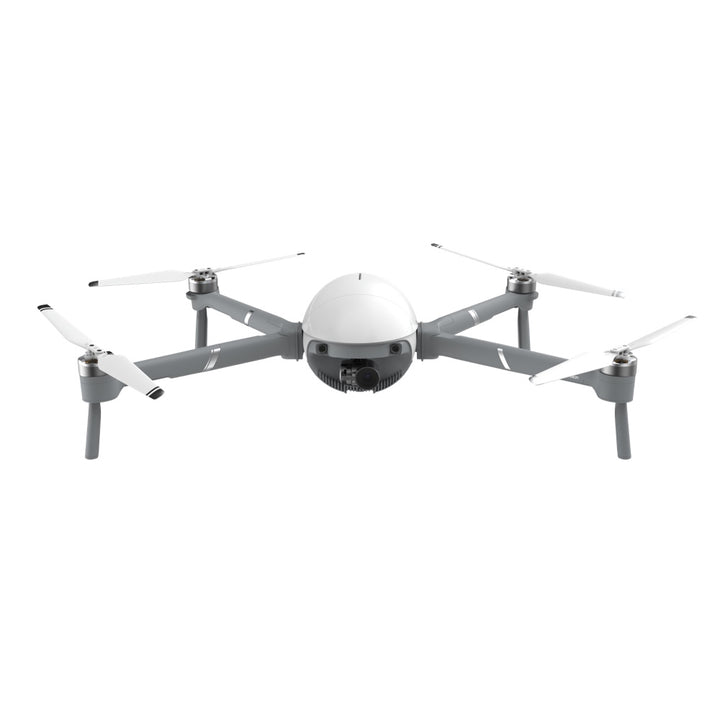
\includegraphics[width=1\linewidth]{uav/models/31_powereggx.jpg}
\caption{PowerEgg X}
\end{wrapfigure}
The PowerEgg X \cite{powereggx} is PowerVision's aerial drone, promoted as a multi-function AI camera.

\paragraph{Payload capacity}\mbox{Score: 0} \\
The payload capacity of the PowerEgg X is not presented on the website and not known from other sources.

\paragraph{Mounting clearance}\mbox{Score: 1.0} \\
The PowerEgg X is a medium sized drone. While it doesn't have special mounting holes, it does have enough clearance on its four horizontal bars

\paragraph{Navigation/Routing}\mbox{Score: 0} \\
While the PowerEgg X does have an app, it doesn't have the ability to set waypoints. Instead, it focuses more on the photography aspects of the drone.

\paragraph{Flight time}\mbox{Score: 1.5} \\
The flight time of the PowerEgg X is 30 minutes, welll passing the minimum required flight time.

\paragraph{Range}\mbox{Score: 1.5} \\
The maximum radio range is 5.9km, well passing the minimum range

\paragraph{Waterproof}\mbox{Score: 1.0} \\
The PowerEgg X has a waterproof kit on the wizard edition. Looking at the specifications, it can be concluded that the drone is rated for IP64 meaning the drone is dust-tight and can sustain splashes. This just meets the minimum required IP rating.

\paragraph{Landing in water}\mbox{Score: 1.3} \\
The PowerEgg X Wizard Edition can land on water with its removable water landing gears

\paragraph{Maneuverability}\mbox{Score: 1.5} \\
The drone can fly horizontally 18m/s. It will recover itself if it is upside down in the water

\paragraph{Total score:}\mbox{0} \\
Due to the PowerEgg X being focused on photography it doesn't have listed payload capacity or the routing capabilities the project needs.


\newpage
\subsubsection{DJI Phantom 4}
\begin{wrapfigure}{r}{0.3\textwidth}
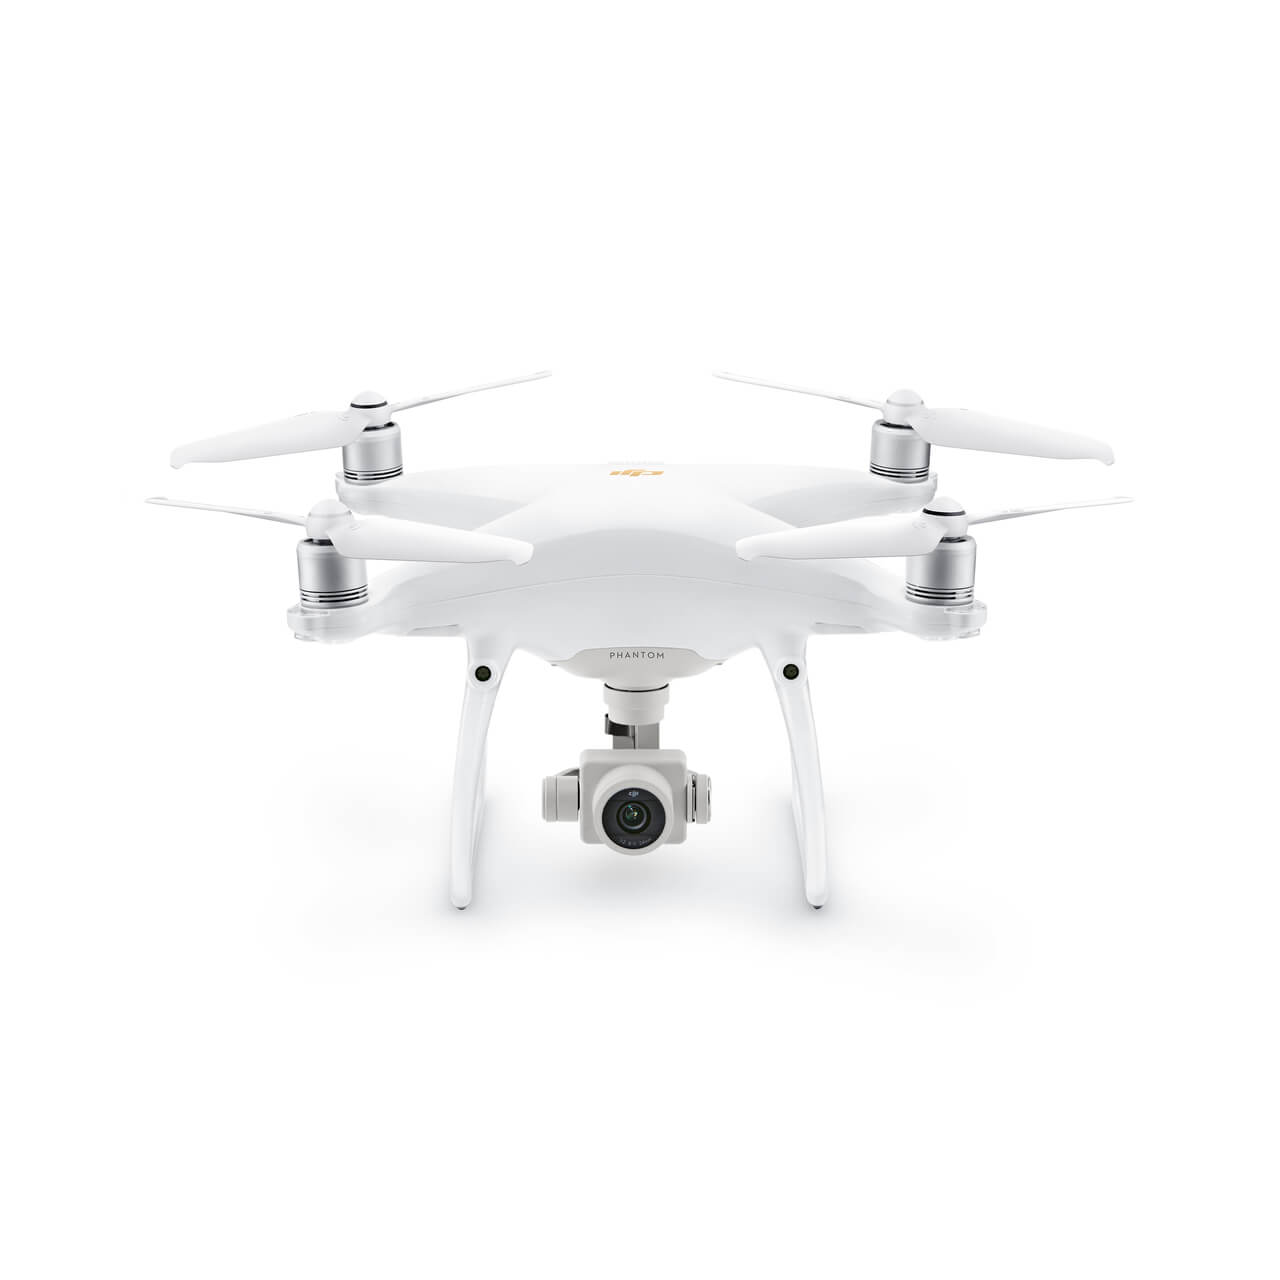
\includegraphics[width=1\linewidth]{uav/models/41_phantom4.jpg}
\caption{Phantom 4}
\end{wrapfigure}
The Phantom 4 \cite{phantom4} was one of DJI's flagship drones. While there have been several variants of this popular drone, like the V2.0 Pro, they are identical to our requirements.

\paragraph{Payload capacity}\mbox{Score: 1.0} \\
While DJI only notes payload capacity on the Matrice 300 Series, the payload capacity of the Phantom 4 is generally considered to be 500 grams. This has been tested by multiple frequent users of the drone. \cite{phantompilots} 

\paragraph{Mounting clearance}\mbox{Score: 1.5} \\
The Phantom 4 is one of the bigger drones. Due to it's popularity, it has several third party mounting solutions that one can buy \cite{polarpro} or build themselves \cite{thingiverse}. One could easily use these mounting solutions to mount sensors or water collectors.

\paragraph{Navigation/Routing}\mbox{Score: 1.5} \\
One can plan routes for the Phantom 4 using the well established DJI Go 4 app \cite{djigo} available on iOS and Android. There is also the excellent DroneExpert search and rescue flight app available on iOS which is designed to pre-program an ideal flight route. \cite{desar}

\paragraph{Flight time}\mbox{Score: 1.3} \\
The flight time of the Phantom 4 is 22 minutes, passing the minimum required flight time.

\paragraph{Range}\mbox{Score: 1.5} \\
The maximum radio range is 5.0km, well over the minimum required range. This also includes image transmission.

\paragraph{Waterproof}\mbox{Score: 1.0} \\
The Phantom 4 is not waterproof by default, but there are wetsuits available which makes the drone dust-tight and immersible up to 1 meter in water, basically creating it IP67 proof. \cite{phantomrain}

\paragraph{Landing in water}\mbox{Score: 0.8} \\
While the Phantom 4 does not have a water landing gear by default, there are commercial kits one can buy to make the drone able to land on water. \cite{buylanding} One could also create their own water landing gear. \cite{diylanding}

\paragraph{Maneuverability}\mbox{Score: 1.4} \\
Because the Phantom 4 is a somewhat bigger drone, it can fly horizontally a maximum of 10m/s. DJI has made sure that even under load the drone is stable.

\paragraph{Total score:}\mbox{4.9} \\
The Phantom 4 seems like a stable option given it's price on the used market and it's popularity in the drone community. DJI's experience in creating drones makes that the drone is less likely to have deal breaking bugs. Replacement parts are also readily available. The downside to this drone is primarily that you will be doing a new project with older hardware that isn't supported by DJI anymore.
\newpage
\subsubsection{DJI Air 2s}
\begin{wrapfigure}{r}{0.3\textwidth}
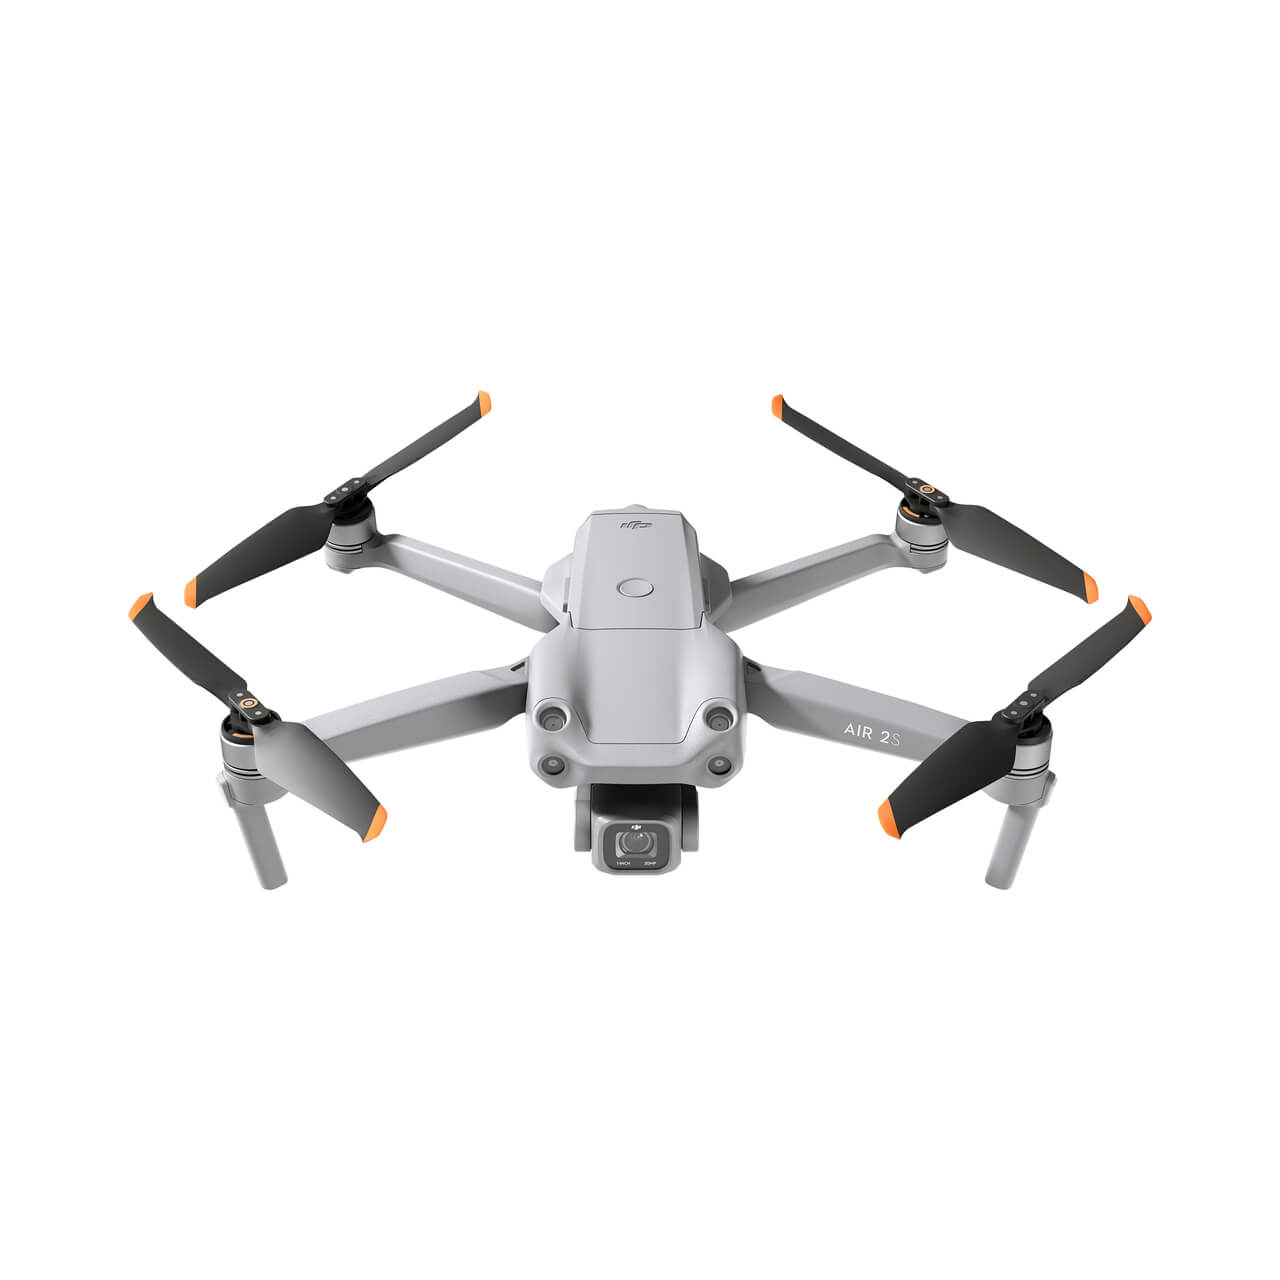
\includegraphics[width=1\linewidth]{uav/models/51_air2s.jpg}
\caption{Air 2S}
\end{wrapfigure}
The Air 2S \cite{phantom4} is DJI's current flagship prosumer drone. While there have been several variants of this popular drone, like the V2.0 Pro, they are identical to our requirements.

\paragraph{Payload capacity}\mbox{Score: 0} \\
While DJI only notes payload capacity on the Matrice 300 Series, the payload capacity of the Phantom 4 is generally considered to be 400 grams. \cite{air2spayloadrelease} This is beneath our minimum requirement of payload capacity.

\paragraph{Mounting clearance}\mbox{Score: 1.0} \\
The Air 2S is a small drone. Due to it's popularity, there does exist  has several third party mounting solutions that one can buy \cite{air2spayloadrelease} or build themselves \cite{thingiverseair}. One could easily use these mounting solutions to mount sensors or water collectors.

\paragraph{Navigation/Routing}\mbox{Score: 1.5} \\
One can plan routes for the Air 2S using the latest DJI Fly app \cite{djifly} available on iOS and Android. There is also the excellent DroneExpert search and rescue flight app available on iOS which is designed to pre-program an ideal flight route. \cite{desar}

\paragraph{Flight time}\mbox{Score: 1.5} \\
The flight time of the Air 2S is 30 minutes, well passing the minimum required flight time.

\paragraph{Range}\mbox{Score: 1.5} \\
The maximum radio range is 12.0km, well over the minimum required range. This also includes image transmission.

\paragraph{Waterproof}\mbox{Score: 1.0} \\
The Air 2S is not waterproof by default, but there are wetsuits available which makes the drone dust-tight and immersible up to 1 meter in water, basically creating it IP67 proof. \cite{air2swetsuit}

\paragraph{Landing in water}\mbox{Score: 0.5} \\
While the Air 2S does not have a water landing gear by default, there are commercial kits one can buy to make the drone able to land on water and give it extra mounting clearance. \cite{air2slandinggear} One could also create their own water landing gear. \cite{diylanding} Because the Air 2S is a smaller drone, it might not be suitable for consistently landing in the water however.

\paragraph{Maneuverability}\mbox{Score: 0.8} \\
The Air 2S is a smaller drone and has the caveats of a smaller drone, being more fragile. It does have the specifications available to go fast, going a maximum of 19m/s.

\paragraph{Total score:}\mbox{0} \\
The Air 2S doesn't seem like a drone suitable for our purposes. The small size makes planned common tasks of the drone quite unstable. It also doesn't meet the payload capacity requirements.

\subsection{Summary of models}

Every drone above is graded by a product of their requirements as seen in \ref{grading}. New and used prices are not included in the score but shown on the bottom of the table. These prices were found as of writing this document (07-03-2022). New prices are resourced from the respective manufacturer's website, while used prices are averaged from eBay \cite{ebay}.

\sffamily\footnotesize
\tabulinesep=6pt
\begin{tabu}{|r|X[cm]|X[cm]|X[cm]|X[cm]|X[cm]|X[cm]|}
\hline
& SplashDrone 4 & Fisherman FD1 & Spry+ & PowerEgg X & Phantom 4 & Air 2S\\
\hline
Payload Capacity   & 1.5 & 1.5 & 0 & 0 & 1.0 & 0\\
Mounting Clearance & 1.3 & 1.1 & 0.8 & 1.0 & 1.5 & 1.0\\
Navigation/Routing & 1.5 & 0.5 & 1.4 & 0 & 1.5 & 1.5\\
Flight time        & 1.5 & 1.5 & 1.5 & 1.5 & 1.3 & 1.5\\
Range              & 1.5 & 1.2 & 0   & 1.5 & 1.5 & 1.5\\
Waterproof         & 1.5 & 1.5 & 1.5 & 1.0 & 1.0 & 1.0\\
Landing in water   & 1.5 & 1.5 & 1.5 & 1.3 & 0.8 & 0.5\\
Maneuverability    & 1.4 & 1.1 & 1.5 & 1.5 & 1.4 & 0.8\\
\hline
Total Score        & 20.7 & 3.7 & 0 & 0 & 4.9 & 0 \\
New Price in EUR   & €2284 & €977 & €903 & €1150 & - & €1300\\
± Used Price in EUR  & €2000 & - & - & €850 & 500 & € 850\\
\hline
\end{tabu}
\rmfamily\normalsize

